\documentclass{article}
\usepackage[T1]{fontenc}
\usepackage{graphicx}
\usepackage{amsmath, amsthm, amssymb}
\usepackage{hyperref}
\usepackage{polski}
\usepackage{listings}
\usepackage{color}
\usepackage{enumerate}
\usepackage{float}
\usepackage{longtable}

\lstset{
	language=C++,
	basicstyle=\ttfamily\footnotesize,
	keywordstyle=\color{blue}\bfseries,
	commentstyle=\color{green},
	stringstyle=\color{red},
	numberstyle=\tiny\color{green},
	numbers=left,
	stepnumber=1,
	tabsize=4,
	breaklines=true,
	showstringspaces=false
}

\begin{document}
	\title{Raport AiSD lista 3}
	\author{Amelia Dorożko}
	\date{\today}
	\maketitle
	
	\section{Problem podziału pręta}
	
	\subsection{\texttt{CUT\_ROD}}
	Funkcja \texttt{CUT\_ROD} jest prostą implementacją algorytmu rekurencyjnego, który rozwiązuje problem cięcia pręta na mniejsze kawałki w sposób "naivny", bez użycia żadnej optymalizacji pamięci.
	
	\subsection{\texttt{MEMORIZED\_CUT\_ROD}}
	Funkcja \texttt{MEMORIZED\_CUT\_ROD} jest ulepszoną wersją funkcji rekurencyjnej, w której zastosowano memoizację. Celem jest unikanie powtarzających się obliczeń, które pojawiają się w naiwnej rekurencji. Zapamiętujemy już obliczone wyniki dla danego $n$ i wykorzystujemy je, gdy są potrzebne ponownie. Chcąc odzyskać rozwiązanie przy użyciu tego algorytmu, korzystamy z poniższej funkcji \texttt{PRINT\_MEMORIZED\_CUT\_ROD}.
	
	\begin{lstlisting}
		void PRINT_MEMORIZED_SOLUTION(int p[], int n) {
			int* r = new int[n + 1];
			fill(r, r + n + 1, -1); // Inicjalizacja tablicy
			
			int maxProfit = MEMORIZED_CUT_ROD(p, r, n);
			cout << "Maksymalny zysk: " << maxProfit << endl;
			
			cout << "Podzial: ";
			while (n > 0) {
				for (int i = 1; i <= n; i++) {
					if (r[n] == p[i-1] + r[n - i]) {
						cout << i << " ";
						n -= i;
						break;
					}
				}
			}
			cout << endl;
			delete[] r;
		}
	\end{lstlisting}
	
	\subsection{\texttt{EXT\_BOT\_UP\_CUT\_ROD}}
	Algorytm \texttt{EXT\_BOT\_UP\_CUT\_ROD} działa na zasadzie programowania dynamicznego. Wykorzystuje podejście bottom-up, co oznacza, że rozwiązanie problemu budowane jest od najprostszych przypadków, aż do przypadków bardziej złożonych. Algorytm przechodzi od najmniejszych problemów (pręt o długości 0) do głównego problemu (pręt o długości $n$), rozwiązując kolejne podproblemy i przechowując wyniki w tablicach, co pozwala uniknąć ich ponownego obliczania. Jego główną zaletą jest możliwość rekonstrukcji rozwiązania, dzięki czemu możemy uzyskać nie tylko optymalny zysk, ale także konkretne cięcia, które prowadzą do tego zysku. Chcąc odzyskać optymalne rozwiązanie, wykorzystujemy funkcję \texttt{ PRINT\_EXT\_SOLUTION}, która korzysta z dwóch tablic zysku i optymalnego podziału.
	
	\begin{lstlisting}
		void PRINT_EXT_SOLUTION(int p[], int n) {
			int* r = new int[n + 1];
			int* s = new int[n + 1];
			
			EXT_BOT_UP_CUT_ROD(p, r, s, n);
			
			cout << "Maksymalny zysk: " << r[n] << endl;
			
			cout << "Podzial: ";
			while (n > 0) {
				cout << s[n] << " ";
				n -= s[n];
			}
			cout << endl;
			
			delete[] r; 
			delete[] s; 
		}
	\end{lstlisting}
	
	\begin{figure}[H]
		\centering
		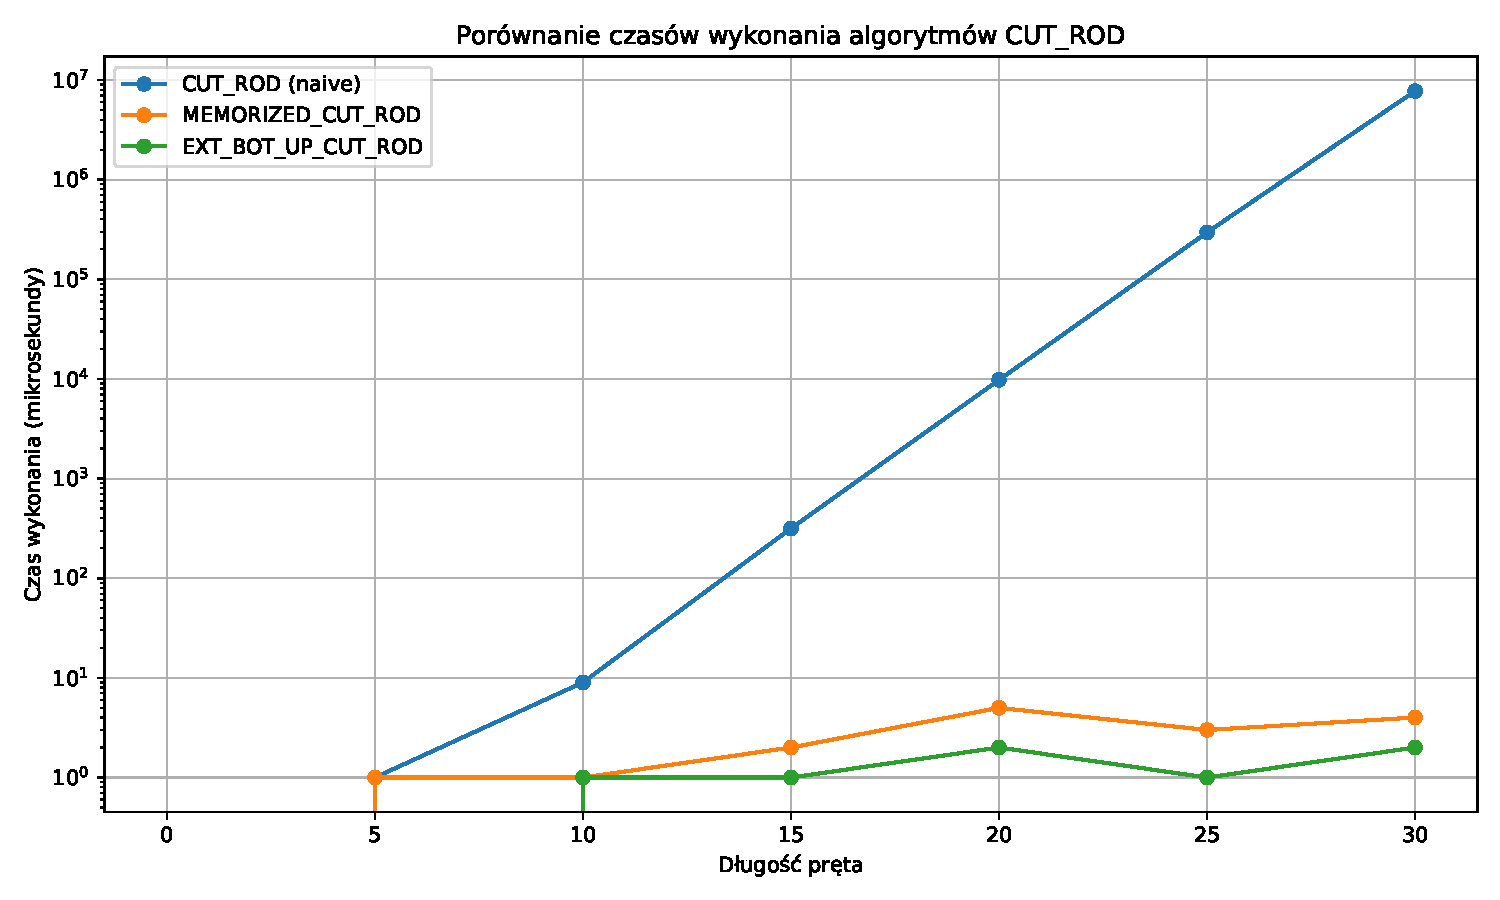
\includegraphics[width=1\textwidth]{wykres1.pdf}
	\end{figure}
	
	Z analizy wynika, że algorytm \texttt{EXT\_BOT\_UP\_CUT\_ROD} działa efektywniej niż pozostałe przy większych danych.
	
	\begin{table}[H]
		\resizebox{\textwidth}{!}{
			\begin{tabular}{|c|c|c|}
				\hline
				\textbf{Długość pręta} & \textbf{MEMORIZED\_CUT\_ROD} & \textbf{EXT\_BOT\_UP\_CUT\_ROD} \\ \hline
				500    & 1496    & 372    \\ \hline
				1000   & 5143    & 1546   \\ \hline
				5000   & 97467   & 33144  \\ \hline
				7000   & 175612  & 62039  \\ \hline
				10000  & 357622  & 143427 \\ \hline
				12000  & 671226  & 195770 \\ \hline
				15000  & 946803  & 305454 \\ \hline
				17000  & 1109070 & 431027 \\ \hline
				20000  & 1597139 & 576887 \\ \hline
				25000  & 2321849 & 811880 \\ \hline
			\end{tabular}
		}
		\caption{Porównanie czasu działania algorytmów, dla danych o większym zakresie (mikrosekundy).}
		\label{tab:large_rod_cutting_times}
	\end{table}
	
	\begin{figure}[H]
		\centering
		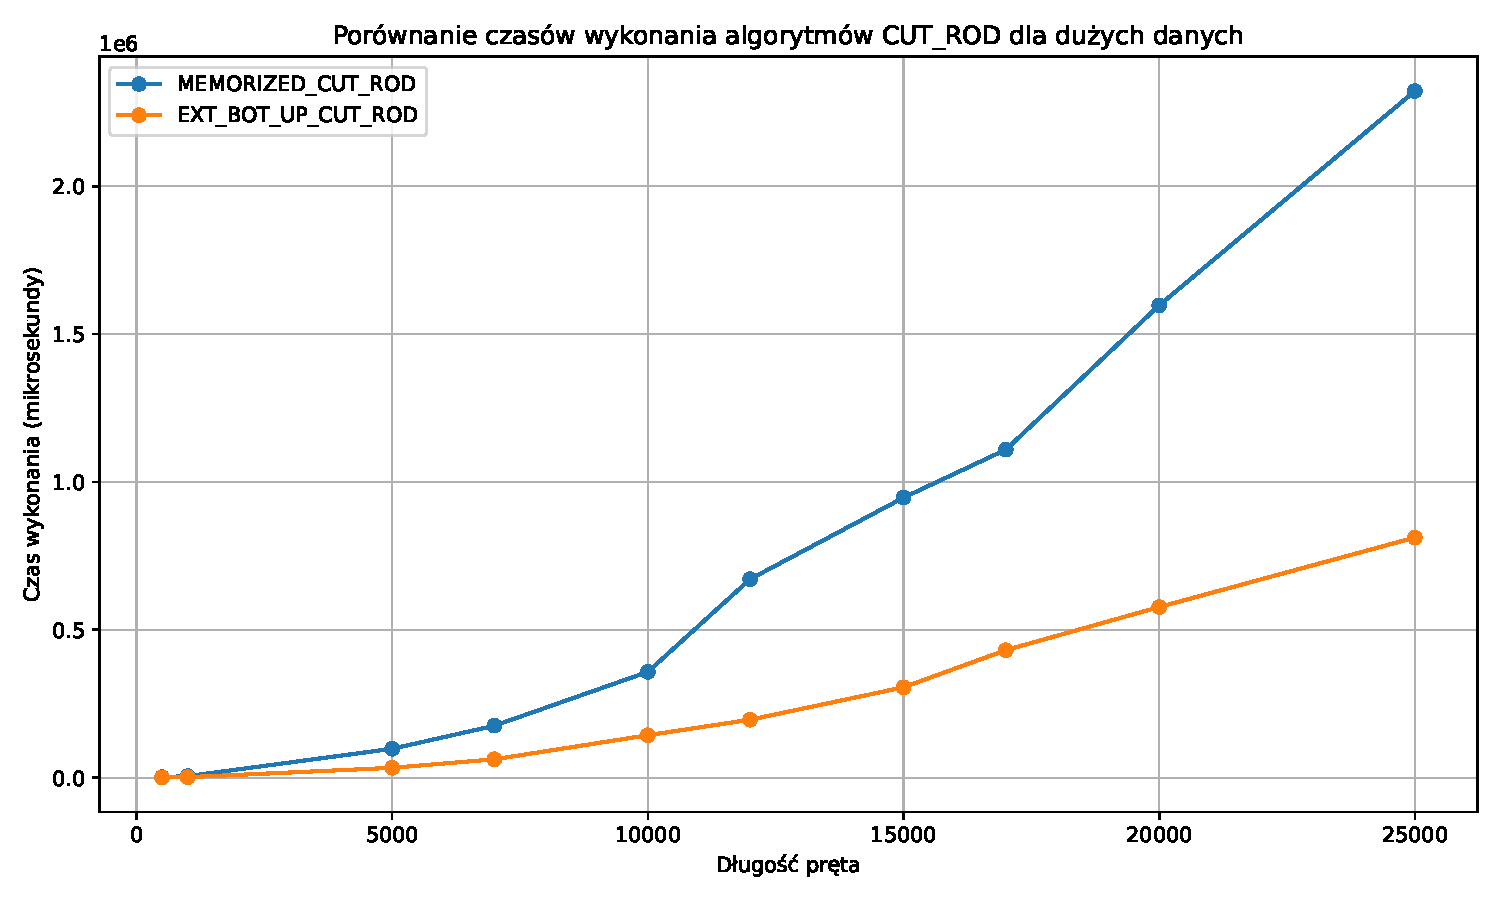
\includegraphics[width=1\textwidth]{wykres2.pdf}
	\end{figure}
	
	Pomimo podobnej złożoności obliczeniowej, algorytmy \texttt{MEMORIZED\_CUT\_ROD} i \texttt{EXT\_BOT\_UP\_CUT\_ROD} różnią się w sposób implementacji. W \texttt{MEMORIZED\_CUT\_ROD} rekurencja wiąże się z wyższym narzutem pamięciowym i czasowym. Z kolei \texttt{EXT\_BOT\_UP\_CUT\_ROD} eliminuje rekurencję, opierając się na podejściu iteracyjnym, co zmniejsza wymagania pamięciowe i poprawia zarządzanie przestrzenią.
	
	Jeśli chodzi o wydajność, dla mniejszych danych różnica jest minimalna, jednak dla większych rozmiarów danych \texttt{EXT\_BOT\_UP\_CUT\_ROD} działa szybciej, ponieważ nie obciąża systemu rekurencją. Dodatkowo, algorytm bottom-up lepiej radzi sobie z większymi problemami i jest bardziej efektywny pod względem pamięciowym.
	
	\section{Najdłuższy wspólny podciąg}

	\subsection{Rekurencyjny algorytm LCS (REC\_LCS)}
	Algorytm rekurencyjny \texttt{REC\_LCS} opiera się na zasadzie podziału problemu na mniejsze podproblemy. Dla dwóch ciągów wejściowych $s1$ i $s2$ o długościach odpowiednio $m$ i $n$, najdłuższy wspólny podciąg można obliczyć rekurencyjnie w następujący sposób:
	\begin{itemize}
		\item Jeśli $m = 0$ lub $n = 0$, najdłuższy wspólny podciąg ma długość 0.
		\item Jeśli ostatnie znaki $s1[m-1]$ i $s2[n-1]$ są takie same, długość LCS jest równa $1 + LCS(m-1, n-1)$.
		\item W przeciwnym razie, długość LCS to $\max(LCS(m-1, n), LCS(m, n-1))$.
	\end{itemize}

	Aby poprawić efektywność, funkcja wykorzystuje technikę memoizacji, przechowując wyniki wcześniejszych wywołań w dynamicznie alokowanej tablicy $b[m][n]$.
	\texttt{REC\_LCS} jest prostym i intuicyjnym do implementacji algorytmem, mimo tego, wymaga dużej liczby rekurencyjnych wywołań, co może czynić go nieefektywnym, ze względu przepełnienia stosu.
	
	\subsection{Iteracyjny algorytm LCS (IT\_LCS)}
	Iteracyjny algorytm (IT\_LCS) korzysta z dynamicznego programowania. Tablica $c[m+1][n+1]$ jest używana do przechowywania długości LCS dla wszystkich możliwych podciągów. Podejście to wypełnia tablicę wiersz po wierszu, stosując następujące zasady:
	\begin{itemize}
		\item Jeśli $X[i-1] = Y[j-1]$, to $c[i][j] = c[i-1][j-1] + 1$.
		\item W przeciwnym przypadku $c[i][j] = \max(c[i-1][j], c[i][j-1])$.
	\end{itemize}
	
	Dodatkowa tablica $b[m][n]$ przechowuje informacje o kierunku, skąd pochodzi optymalne rozwiązanie (\texttt{'\\'}, \texttt{'|'}, \texttt{'-'}).

	
	
Dla dużych danych wejściowych algorytm iteracyjny działa znacznie szybciej niż rekurencyjny, co czyni go bardziej odpowiednim dla zastosowań praktycznych.
	\begin{table}[H]
		\resizebox{\textwidth}{!}{
		\centering
		\begin{tabular}{|c|c|c|c|c|}
			\hline
			\textbf{Długość ciagów} & \textbf{Czas rekurencyjny (mikrosekundy)} & \textbf{Czas iteracyjny (mikrosekundy)} \\ \hline
			100   & 281    & 246    \\ \hline
			1000  & 34384  & 12813  \\ \hline
			2000  & 134854 & 64630  \\ \hline
			3000  & 191414 & 94692  \\ \hline
			4000  & 431470 & 271382 \\ \hline
			5000  & 625166 & 260978 \\ \hline
			6000  & 785324 & 467062 \\ \hline
			7000  & 1218602 & 497589 \\ \hline
			8000  & 1305638 & 633539 \\ \hline
			9000  & 1585806 & 927642 \\ \hline
			10000 & 1963625 & 1190042 \\ \hline
		\end{tabular}
	}
		\caption{Porównanie czasów wykonania algorytmu rekurencyjnego i iteracyjnego LCS dla różnych długości ciągów.}
		\label{tab:lcs_comparison}

	\end{table}
	
	
	Dla małych danych algorytm \texttt{REC\_LCS} może być szybszy, ponieważ wymaga mniejszej pamięci, nie musi tworzyć dużych tablic, a sama liczba obliczeń jest wystarczająco mała, by działać efektywnie. Co przedstawia wykres dla mniejszego zakresu napisów.
	
	\begin{figure}[H]
	\centering
	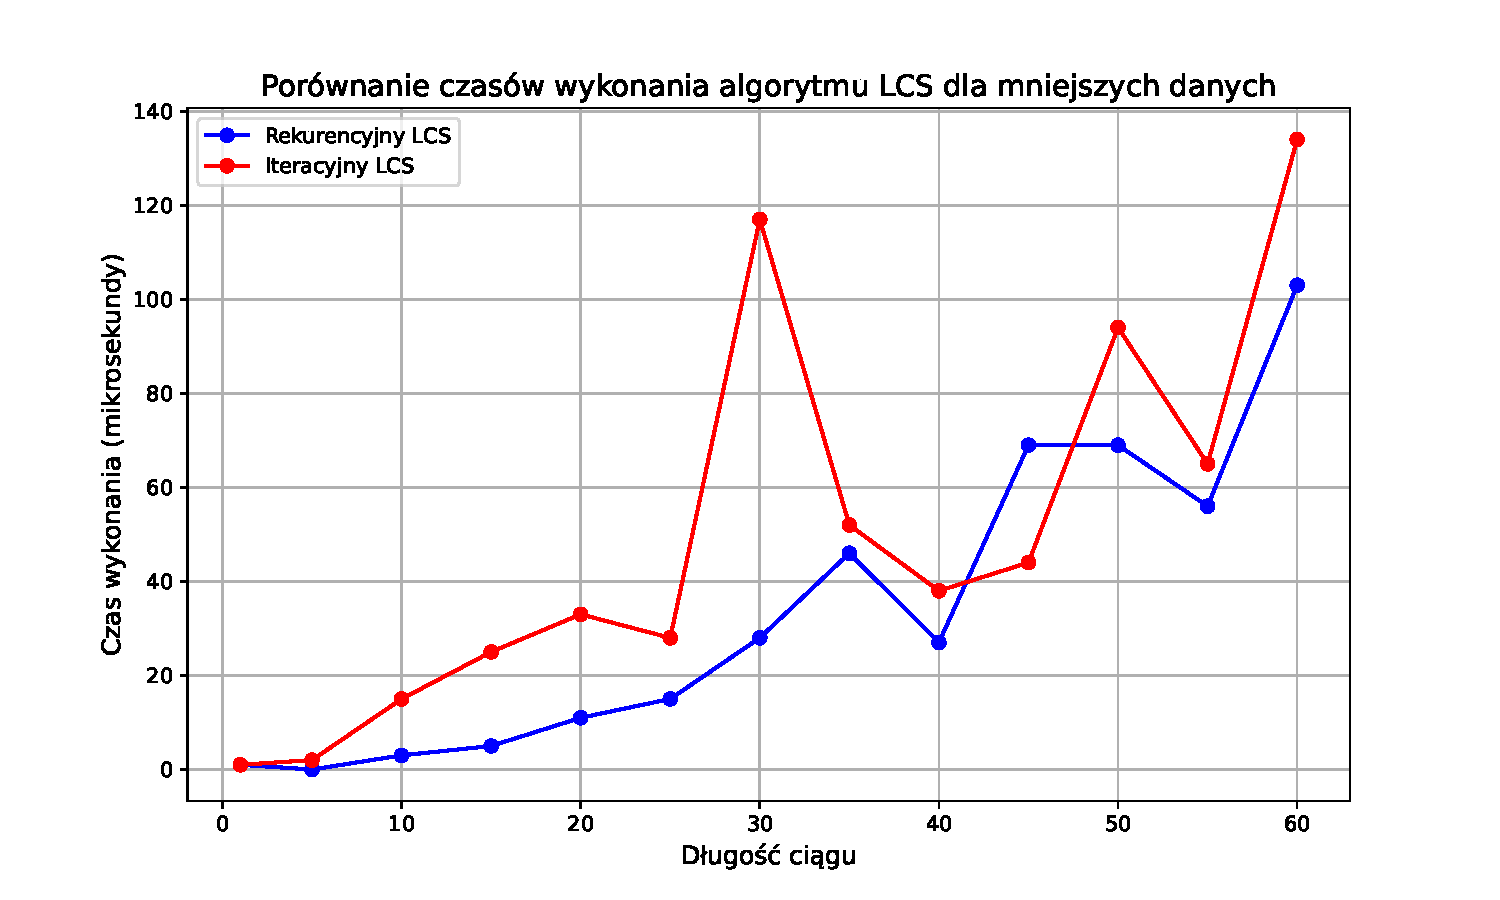
\includegraphics[width=1\textwidth]{wykres4.pdf}
	\end{figure}
	
	Z kolei dla większych danych jego wydajność spada, gdyż nie używa pamięci do zapisywania wyników pośrednich, co prowadzi do wielu powtórzeń obliczeń. W takich przypadkach algorytm iteracyjny jest bardziej efektywny.
	
		\begin{figure}[H]
		\centering
		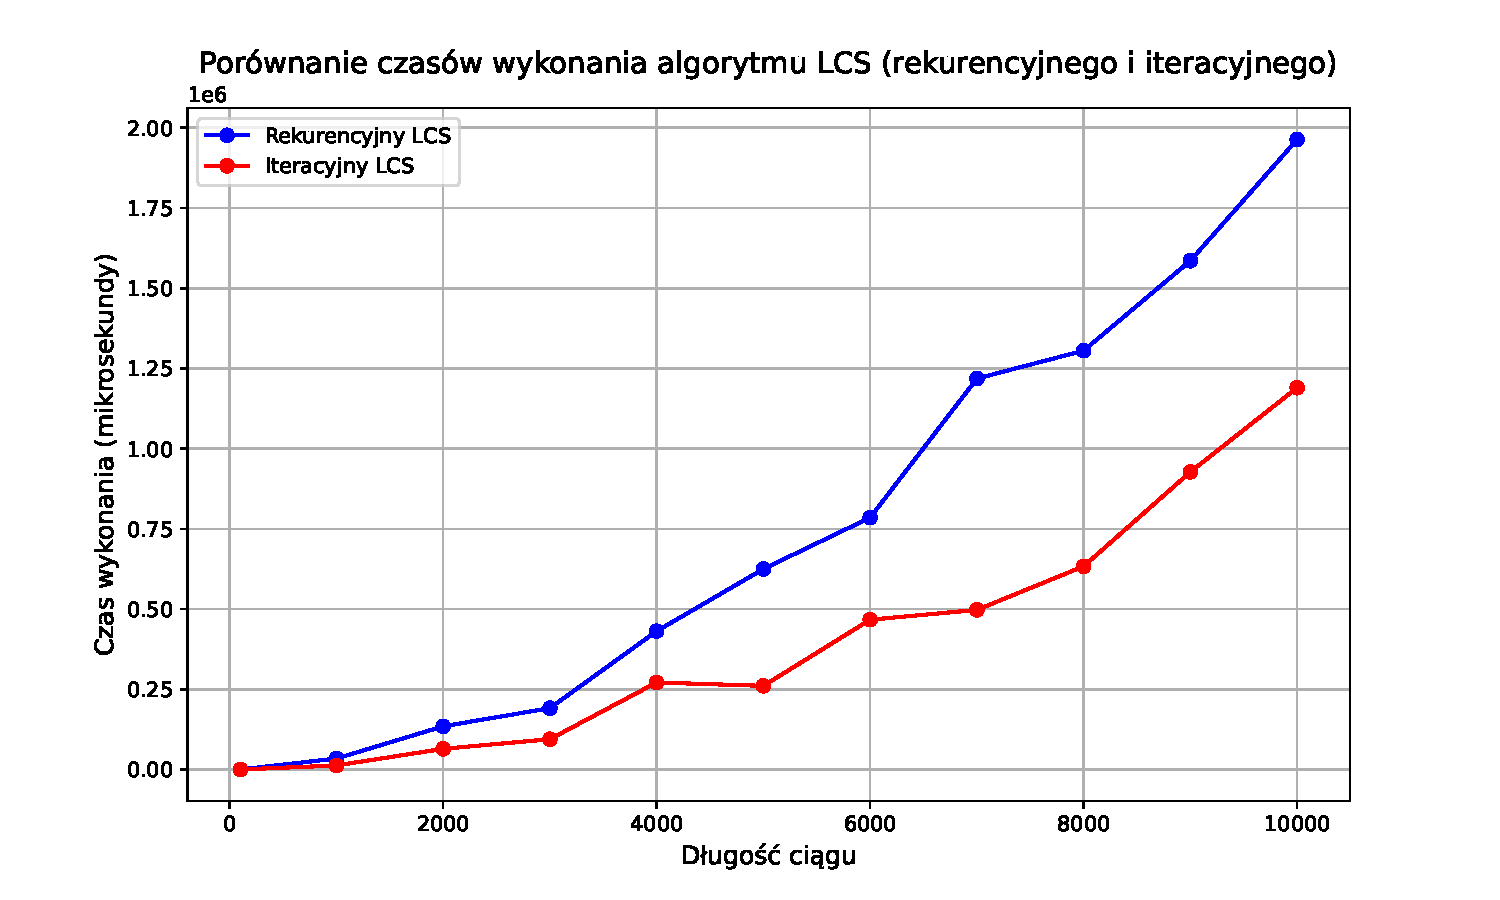
\includegraphics[width=1\textwidth]{wykres3.pdf}
	\end{figure}
	\section{Problem wyboru zajęć}
	\subsection{Algorytmy z posortowaną tablicą \texttt{f[]}}
	Funkcje \texttt{F\_RECURSIVE\_ACTIVITY\_SELECTOR} oraz \texttt{F\_ACTIVITY\_SELECTOR} działają dla posortowanej tablicy zakończenia zajęć \texttt{f[]}. Te algorytmy selekcjonują możliwe zajęcia, które mogą się odbyć w określonym czasie, bazując na porównaniu czasów rozpoczęcia z czasami zakończenia. 
	
	Funkcja \texttt{F\_RECURSIVE\_ACTIVITY\_SELECTOR} używa rekurencji. Początkowy indeks \texttt{k} jest równy 0. Algorytm zaczyna iterację od kolejnego możliwego zajęcia \texttt{s[m]}, sprawdzając, czy jego czas rozpoczęcia jest większy lub równy czasowi zakończenia zajęcia \texttt{f[k]}. Jeśli tak, to dane zajęcia są wybierane, a rekurencja kontynuuje dla \texttt{m}. 
	
	Funkcja \texttt{F\_ACTIVITY\_SELECTOR} działa iteracyjnie. Zaczynamy od pierwszego zajęcia (indeks 1), zapamiętujemy je jako wybrane. W kolejnych krokach algorytm sprawdza, czy czas rozpoczęcia zajęcia \texttt{s[m]} jest większy lub równy czasowi zakończenia zajęcia \texttt{f[k]}. Jeśli tak, to zajęcia są wybierane, a indeks \texttt{k} zostaje zaktualizowany.
		\begin{figure}[H]
		\centering
		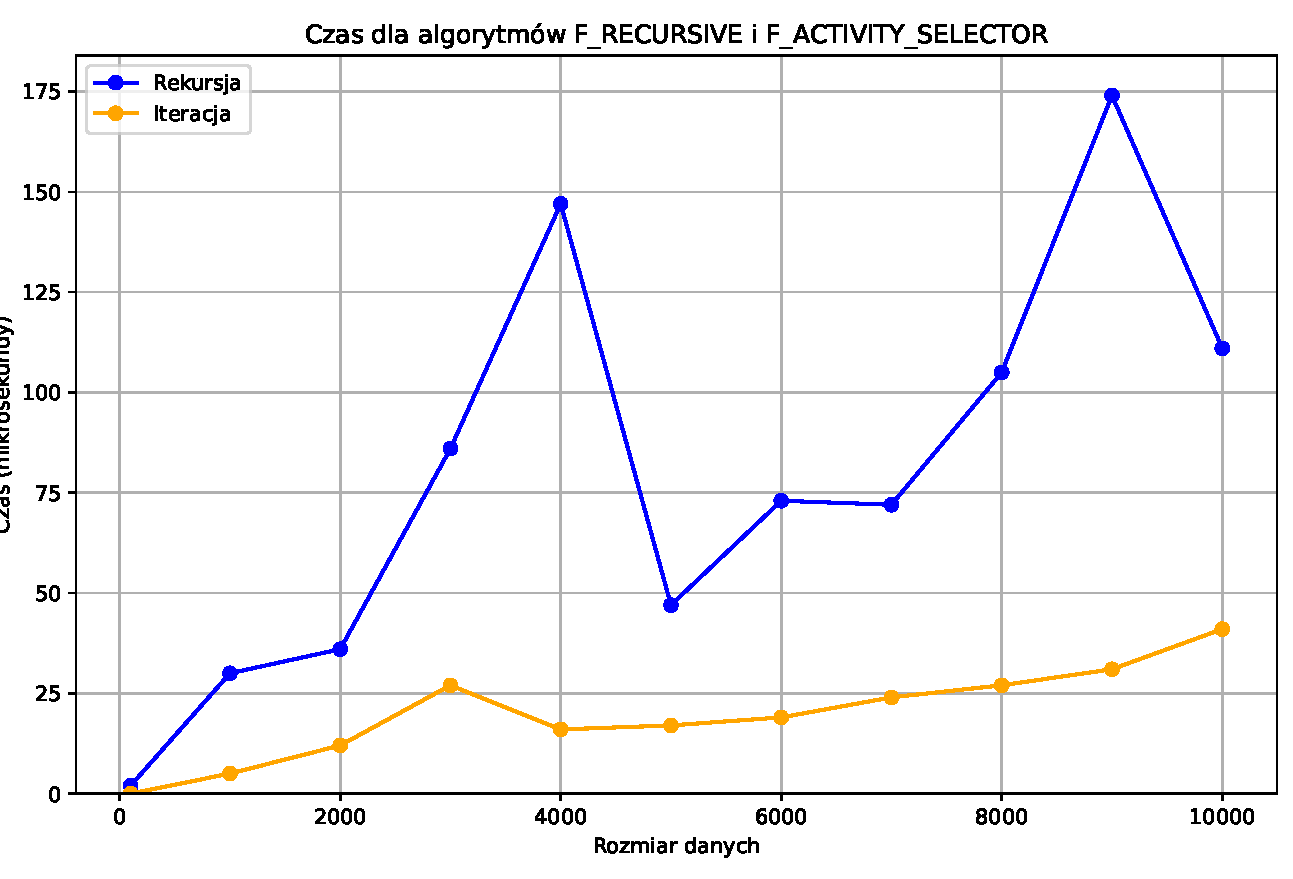
\includegraphics[width=0.8\textwidth]{wykres6.pdf}
	\end{figure}
	
	\subsection{Algorytmy z posortowaną tablicą \texttt{s[]}}
	
	Funkcje \texttt{S\_RECURSIVE\_ACTIVITY\_SELECTOR} oraz \texttt{S\_ACTIVITY\_SELECTOR} działają dla posortowanej tablicy rozpoczęcia zajęć \texttt{s[]}. Te algorytmy selekcjonują zajęcia, które mogą się rozpocząć po zakończeniu wcześniejszych zajęć. 
	
	Funkcja \texttt{S\_RECURSIVE\_ACTIVITY\_SELECTOR} działa rekurencyjnie. Rozpoczyna iterację od ostatniego zajęcia i sprawdza, czy czas zakończenia zajęcia \texttt{f[m]} jest większy od czasu rozpoczęcia zajęcia \texttt{s[k]}. Jeśli tak, to indeks \texttt{m} zostaje zaktualizowany, a rekurencja kontynuuje.
	
	Funkcja \texttt{S\_ACTIVITY\_SELECTOR} działa iteracyjnie. Zaczynamy od ostatniego zajęcia (indeks n-1) i zapamiętujemy je jako wybrane. Algorytm sprawdza, czy czas zakończenia zajęcia \texttt{f[m]} jest mniejszy lub równy czasowi rozpoczęcia zajęcia \texttt{s[k]}. Jeśli tak, to dane zajęcia są wybierane, a indeks \texttt{k} zostaje zaktualizowany.
	
		
		\subsubsection*{Przykładowe rozwiązanie z posortowaną tablicą \texttt{s[]}}
	
	\begin{table}[H]
		\centering
		\begin{tabular}{|c|c|c|}
			\hline
			\textbf{Zajęcie} & \textbf{Czas rozpoczęcia} & \textbf{Czas zakończenia} \\ \hline
			1 & 6 & 15 \\ \hline
			2 & 10 & 18 \\ \hline
			3 & 18 & 28 \\ \hline
			4 & 20 & 23 \\ \hline
			5 & 30 & 34 \\ \hline
			6 & 33 & 42 \\ \hline
			7 & 37 & 45 \\ \hline
			8 & 45 & 55 \\ \hline
			9 & 46 & 53 \\ \hline
		\end{tabular}
		\caption{Dostępne zajęcia z ich czasami rozpoczęcia i zakończenia.}
	\end{table}
	
	\subsubsection*{Wynik algorytmów}
	
	\subsubsection*{Metoda rekurencyjna}
	Wybrane zajęcia (w kolejności wyboru): \(2, 4, 5, 7, 9\).
	\subsubsection*{Metoda iteracyjna}
	Wybrane zajęcia (w kolejności wyboru): \(2, 4, 5, 7, 9\).

	\subsubsection*{Dynamiczne rozwiązanie problemu}
	Funkcja \texttt{DYNAMIC\_A\_S} realizuje algorytm selekcji aktywności dynamicznej, który wybiera maksymalną liczbę aktywności, nie nakładających się na siebie. 

	Funkcja \texttt{DYNAMIC\_A\_S} korzysta z dwóch tablic:
	\begin{itemize}
		\item \texttt{dp}: Tablica przechowująca maksymalną liczbę aktywności do danego momentu.
		\item \texttt{prev}: Tablica przechowująca indeks poprzedniej aktywności w optymalnym rozwiązaniu.
	\end{itemize}
	Algorytm iteracyjnie przechodzi przez wszystkie aktywności, korzystając z funkcji \texttt{last}, która znajduje ostatnią aktywność nie nakładającą się na aktualną. Wynik jest wyświetlany w postaci wybranych aktywności.
	
	Poniżej przedstawiono kod funkcji \texttt{DYNAMIC\_A\_S}:
	\begin{lstlisting}
	
		int last(int s[], int f[], int i) {
			for (int j = i - 1; j >= 0; j--) {
				if (f[j] <= s[i]) {
					return j;
				}
			}
			return -1;
		}
		
		void DYNAMIC_A_S(int s[], int f[], int n) {
			int dp[n];
			int prev[n];
			dp[0] = 1;
			prev[0] = 0;
			
			for (int i = 1; i < n; i++) {
				int k = last(s, f, i);
				if (k != -1 && dp[k] + 1 > dp[i - 1]) {
					dp[i] = dp[k] + 1;
					prev[i] = i;
				} else {
					dp[i] = dp[i - 1];
					prev[i] = prev[i - 1];
				}
			}
			
			cout << "Wybrane zajecia:\n";
			int i = n - 1;
			while (i > 0) {
				if (prev[i] == i) {
					cout << "(" << s[i] << ", " << f[i] << ") ";
					i = last(s, f, i);
				} else {
					i--;
				}
			}
	\end{lstlisting}
	Porównując z poprzednimi algorytmami, dynamiczne podejście do problemu nie jest optymalne.
		\begin{figure}[H]
		\centering
		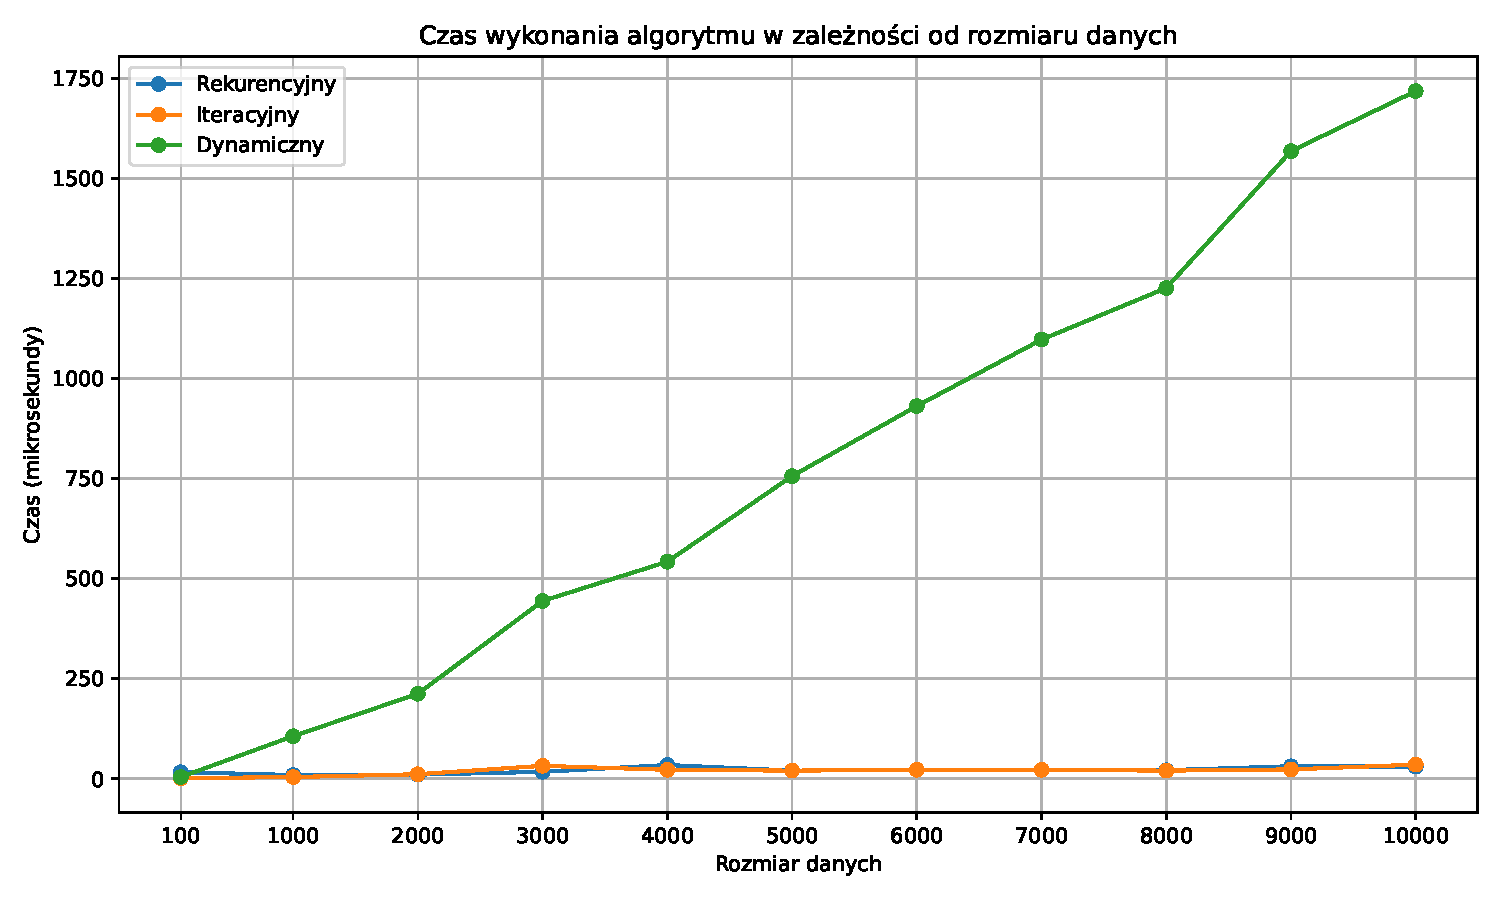
\includegraphics[width=1\textwidth]{wykres8.pdf}
	\end{figure}
	W każdym przypadku algorytmy działają dla posortowanej listy zajęć i dokonują selekcji zgodnie z określonym kryterium, czy to czasu zakończenia \(f[]\) czy rozpoczęcia \(s[]\).
		\begin{figure}[H]
		\centering
		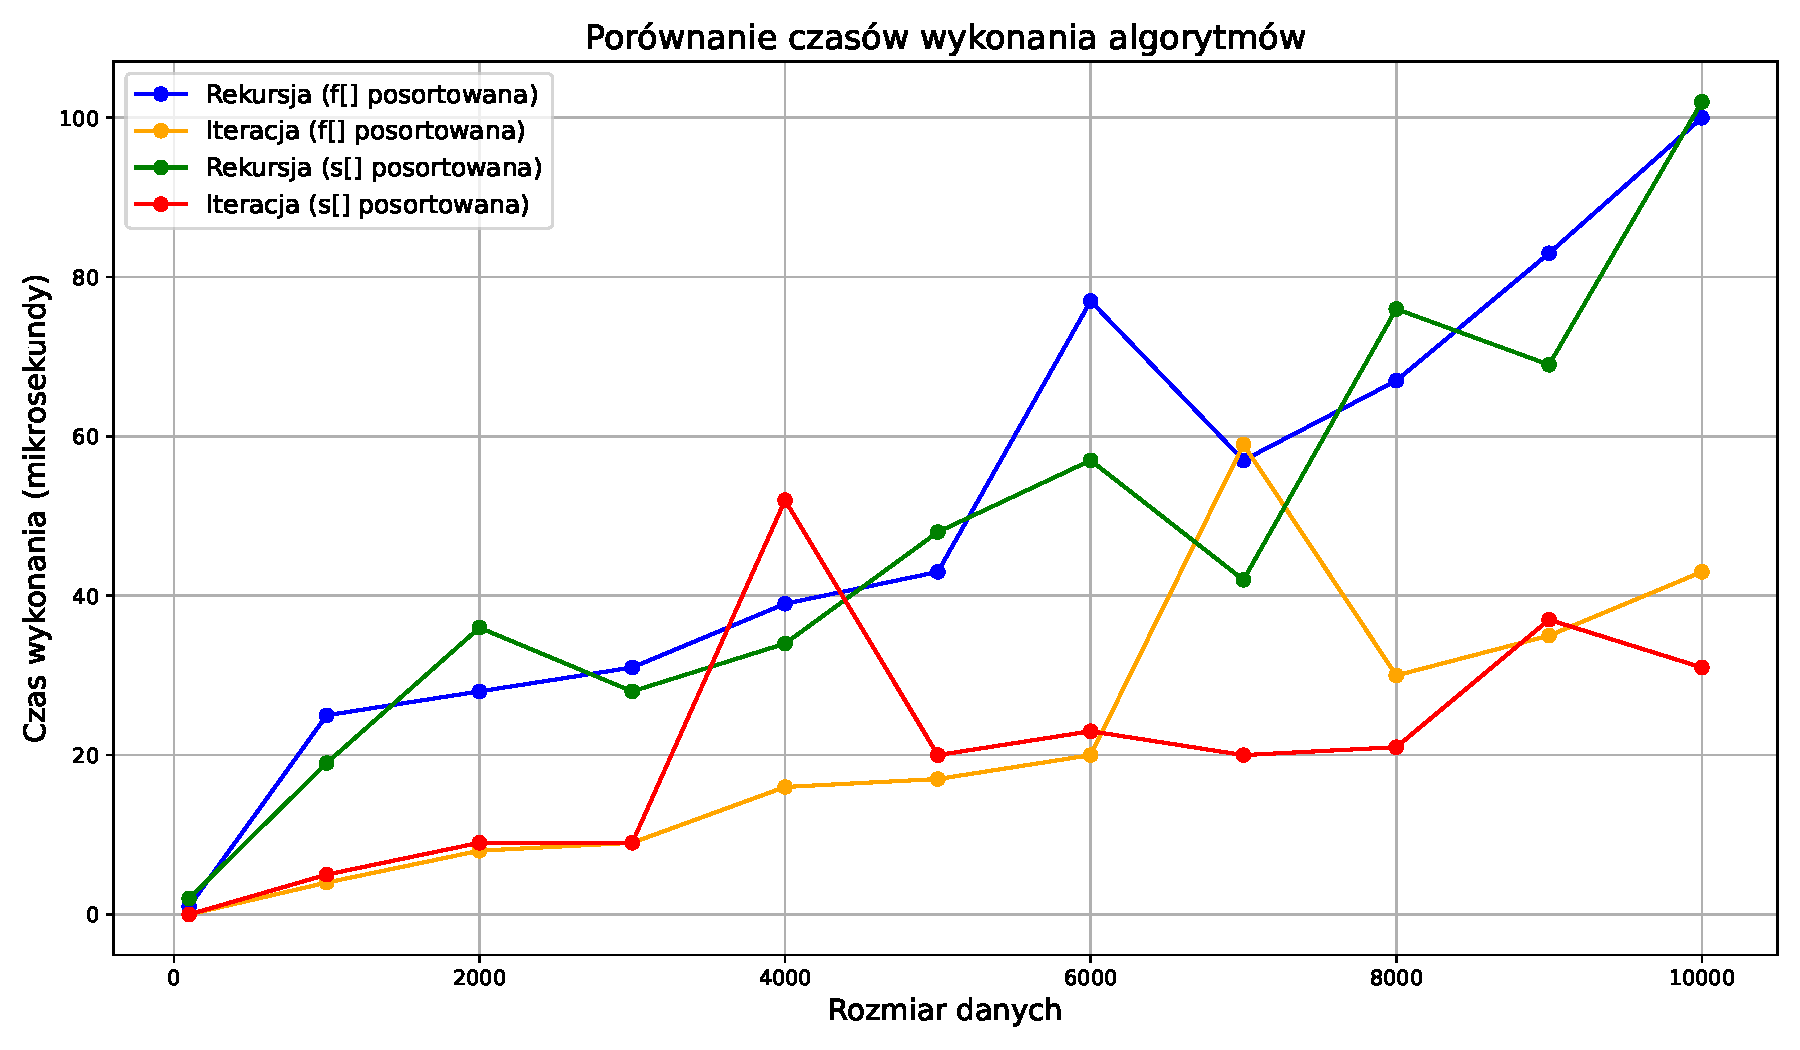
\includegraphics[width=1\textwidth]{wykres7.pdf}
	\end{figure}
	



\end{document}
